\begin{exercises} 

\item Respond to each of the following prompts to solve the given optimization problem.
\ba
  \item Let  $f(x,y) = \sin(x)+\cos(y)$. Determine the absolute maximum and minimum values of $f$. At what points do these extreme values occur?

  \item For a certain differentiable function $F$ of two variables $x$ and $y$, its partial derivatives are 
$$F_x(x,y) = x^2-y-4 \ \ \mbox{and} \ \ F_y(x,y) = -x + y - 2.$$  Find each of the critical points of $F$, and classify each as a local maximum, local minimum, or a saddle point. 

  \item Determine all critical points of $T(x,y) = 48 + 3xy - x^2y - xy^2$ and classify each as a local maximum, local minimum, or saddle point.
  
  \item Find and classify all critical points of  $g(x,y) = \frac{x^2}{2} + 3y^3 + 9y^2 - 3xy + 9y - 9x$

  \item Find and classify all critical points of $z = f(x,y) = ye^{-x^2-2y^2}$.
  
  \item Determine the absolute maximum and absolute minimum of $f(x,y) = 2 + 2x + 2y - x^2 - y^2$ on the triangular plate in the first quadrant bounded by the lines $x = 0$, $y = 0$, and $y = 9-x$.

  \item Determine the absolute maximum and absolute minimum of $f(x,y) = 2 + 2x + 2y - x^2 - y^2$ over the closed disk of points $(x,y)$ such that $(x-1)^2 + (y-1)^2 \le 1$.
  
  \item Find the point on the plane $z = 6 - 3x - 2y$ that lies closest to the origin.

\ea

\begin{exerciseSolution}
\ba
  \item We want to determine when $f_x(x,y)$ and $f_y(x,y)$ are simultaneously 0. Now $f_x(x,y) = \cos(x)$ and $f_y(x,y) = -\sin(y)$ are 0 when $x = \frac{\pi}{2} + k \pi$ and $y = m \pi$, where $k$ and $m$ are integers. We know that $\sin\left(\frac{\pi}{2} + k \pi\right)$ is either 1 or $-1$ depending on whether $k$ is even or odd, respectively, and $\cos(m \pi)$ is also 1 or $-1$ depending on whether $m$ is even or odd, respectively. It follows that $f\left(\frac{\pi}{2} + k \pi, m \pi\right)$ is $-2$, $0$, or $2$. So the maximum value of $f$ is 2, which occurs when $x = \frac{\pi}{2} + k \pi$ and $y = m \pi$ for $k$ and $m$ even. Also, the minimum value of $f$ is $-2$, which occurs when $x = \frac{\pi}{2} + k \pi$ and $y = m \pi$ for $k$ and $m$ odd. 

  \item Since $F_x$ and $F_y$ exist everywhere, the critical points of $F$ occur when $F_x(x,y)$ and $F_y(x,y)$ are simultaneously 0. We solve the system
\begin{align*}
x^2-y-4 &= 0 \\
-x + y - 2 &= 0
\end{align*}
by substituting $y = x+2$ into the first equation. This leads to the critical points $(3,5)$ and $(-2,0)$. We use the Second Derivative Test to classify these critical points. Note that 
\[F_{xx}(x,y) = 2x, \ F_{yy}(x,y) = 1, \ \text{ and } \ F_{xy}(x,y) = -1.\]
Since $F_{xx}(3,5)F_{yy}(3,5) - F_{xy}(3,5)^2 = 5 > 0$ and $F_{xx}(3,5) = 6 > 0$, it follows that $F$ has a local minimum at $(3,5)$. Also, $F_{xx}(-2,0)F_{yy}(-2,0) - F_{xy}(-2,0)^2 = -5 <  0$ tells us that $F$ has a saddle point at $(-2,0)$. 

  \item We find the points at which $T_x(x,y)$ and $T_y(x,y)$ are simultaneously 0. To solve the system
\begin{align*}
T_x(x,y) &= 3y-2xy-y^2 = 0 \\
T_y(x,y) &= 3x-x^2-2xy = 0 
\end{align*}
we subtract the second equation from the first leaving us with 
\[0 = 3y-y^2-3x+x^2 = 3(y-x) - (y-x)(y+x) = (y-x)(3-y-x).\]
So either $y=x$ or $y=3-x$. If $y=x$, then the first equation tells us that $0 = 3x-3x^2 = 3x(1-x)$. In this case we have the critical points $(0,0)$ and $(1,1)$. If $y=3-x$, the second equation tells us that $0 = 3x-x^2-2(3-x) = x(x-3)$. In this case we have critical points $(3,0)$ and $(0,3)$.

We use the Second Derivative Test to classify these critical points. Here we have 
\[T_{xx}(x,y) = -2y, \ T_{yy}(x,y) = -2x, \ \text{ and } \ T_{xy}(x,y) = 3-2x-2y.\]

\begin{itemize}
\item Since $T_{xx}(0,0)T_{yy}(0,0) - T_{xy}(0,0)^2 = -3 < 0$, the function $T$ has a saddle point at $(0,0)$.
\item Since $T_{xx}(1,1)T_{yy}(1,1) - T_{xy}(1,1)^2 = 3 > 0$ and $T_{xx}(1,1) < 0$, the function $T$ has a relative maximum at $(1,1)$.
\item Since $T_{xx}(3,0)T_{yy}(3,0) - T_{xy}(3,0)^2 = -16 < 0$, the function $T$ has a saddle point at $(3,0)$.
\item Since $T_{xx}(0,3)T_{yy}(0,3) - T_{xy}(0,3)^2 = -16 < 0$, the function $T$ has a saddle point maximum at $(0,3)$.
\end{itemize}

  
  \item In this example we have 
\[g_x(x,y) = x-3y - 9 \ \text{ and } \ g_y(x,y) = 9y^2+18y-3x+9.\]
Solving $g_x(x,y)=0$ for $x$ and substituting into $g_y(x,y) = 0$ gives us the equation $9y^2+18y-3(3y-9)+9 = 0$ with solutions $y=-2$ and $y=1$. The corresponding critical points are $(3,-2)$ and $(12,1)$. 

We use the Second Derivative Test to classify these critical points. Here we have 
\[g_{xx}(x,y) = 1, \ g_{yy}(x,y) = 18y+18, \ \text{ and } \ g_{xy}(x,y) = -3.\]

\begin{itemize}
\item Since $g_{xx}(3,-2)g_{yy}(3,-2) - g_{xy}(3,-2)^2 = -27 < 0$, the function $g$ has a saddle point at $(3,-2)$.
\item Since $g_{xx}(12,1)g_{yy}(12,1) - g_{xy}(12,1)^2 = 27 > 0$ and $g_{xx}(12,1) > 0$, the function $g$ has a relative minimum at $(12,1)$.
\end{itemize}



  \item For this function we 
\[f_x(x,y) = -2xye^{-x^2-2y^2} \ \text{ and } \ f_y(x,y) = e^{-x^2-2y^2}-4y^2e^{-x^2-2y^2} = e^{-x^2-2y^2}(1-4y^2).\]
Since $e^{-x^2-2y^2}$ is never 0, the only way both $f_x(x,y)=0$ and $f_y(x,y) = 0$ is if $-2xy=0$ and $1-4y^2=0$. This makes $y = \pm \frac{1}{2}$ and $x=0$, giving us two critical points $\left(0, -\frac{1}{2}\right)$ and $\left(0, \frac{1}{2}\right)$. 

We use the Second Derivative Test with 
\[f_{xx}(x,y) = 4x^2ye^{-x^2-2y^2} - 2ye^{-x^2-2y^2}, \ f_{yy}(x,y) = -12ye^{-x^2-2y^2}+16y^3e^{-x^2-2y^2}, \ \text{ and } \ f_{xy}(x,y) = -2xe^{-x^2-2y^2}+8y^2xe^{-x^2-2*y^2}.\]
to classify these critical points. 
\begin{itemize}
\item Since $f_{xx}\left(0,-\frac{1}{2}\right)f_{yy}\left(0,-\frac{1}{2}\right) - f_{xy}\left(0,-\frac{1}{2}\right)^2 = 4\left(e^{-1/2}\right)^2 > 0$ and $f_{xx}\left(0,-\frac{1}{2}\right) = e^{-1/2}$, the function $g$ has a relative minimum at $\left(0,-\frac{1}{2}\right)$. 
\item Since $f_{xx}\left(0,\frac{1}{2}\right)f_{yy}\left(0,\frac{1}{2}\right) - f_{xy}\left(0,\frac{1}{2}\right)^2 = 4\left(e^{-1/2}\right)^2 > 0$ and $f_{xx}\left(0,\frac{1}{2}\right) = -e^{-1/2}$, the function $g$ has a relative maximum at $\left(0,-\frac{1}{2}\right)$. 
\end{itemize}


  
  \item First we find the critical points of $f$ on the triangular domain. The first order partial derivatives of $f$ are 
\[f_x(x,y) = 2-2x \ \text{ and } \ f_y(x,y) = 2 - 2y.\]
So $f_x(x,y) = 0$ and $f_y(x,y) = 0$ when $x=1$ and $y=1$, giving us a single critical point $(1,1)$. This point is in the first quadrant and satisfies $y < 9-x$, so is in our domain. 

Next we check the boundaries $x=0$ for $0 \leq y \leq 9$, $y=0$ for $0 \leq y \leq 9$, and $y=9-x$ for $0 \leq x \leq 9$. 
\begin{itemize}
\item When $x=0$ we have $f(0,y) = 2+2y-y^2$. Since $f'(y) = 2-2y$, the only critical point of $f$ is $(0,1)$. The endpoints of this portion of the boundary are $(0,0)$, and $(0,9)$, which we also need to check.
\item When $y=0$ we have $f(x,0) = 2+2x-x^2$. Since $f'(x) = 2-2x$, the only critical point of $f$ is $(1,0)$. The endpoints of this portion of the boundary are $(0,0)$, and $(9,0)$, which we also need to check.
\item When $y=9-x$ we have $f(x,9-x) = 2+2x+2(9-x)-x^2-(9-x)^2$. Since $f'(x) = -2x+2(9-x) = -4x+18$, the only critical point of $f$ is $(4.5,4.5)$ The endpoints of this portion of the boundary are $(0,0)$, and $(0,9)$, which we also need to check.
\end{itemize}
Now we test $f$ at the critical points and the appropriate points on the boundary:
\[f(1,1) = 4, \ f(0,0)=2, \ f(0,9) = -61, \ f(9,0) = -61, \ f(0,1) = 3, \ f(1,0)=3, \ \text{ and } \ f(4.5,4.5) = -20.5.\]
So the absolute maximum value of $f$ on this domain is 4 and the absolute minimum value is $-61$. 	


  \item This is the same function as in the previous part of the problem, so the single critical point of $f$ is $(1,1)$. Now we check the boundary. We can parameterize the boundary of the disk by $x(t) = \cos(t)+1$ and $y(t)=\sin(t)+1$. On this boundary we have $f(\cos(t)+1, \sin(t)+1) = 3$. Since $f(1,1) = 4$, it follows that the maximum value of $f$ on this disk is 4 and the minimum value is 3. 
  
  \item A point on the plane has coordinates $(x,y,6-3x-2y)$, so the distance from the origin to a point $(x,y,z)$ on the plane is 
\[d(x,y) = \sqrt{x^2+y^2+(6-3x-2y)^2}.\]
We want to find the minimum value of $d$. Since $d$ cannot be negative, the minimum value of $d$ will occur at the same point as the minimum value of $f(x,y)=d^2(x,y) = x^2+y^2+(6-3x-2y)^2$. Now
\[f_x(x,y) = 2x-6(6-3x-2y) = 20x+12y-36 \ \text{ and } \ f_y(x,y) =  2y-4(6-3x-2y) = 12x+10y-24.\]
To solve the system $f_x(x,y)=0$ and $f_y(x,y)=0$, we use elimination to obtain the critical point $\left(\frac{9}{7}, \frac{6}{7}\right)$. Now 
$f_{xx}(x,y)f_{yy}(x,y) - f_{xy}(x,y)^2 = 56 > 0$ and $f_{xx}(x,y) = 20 > 0$, so the surface is always concave up. This demonstrates that the point $\left(\frac{9}{7}, \frac{6}{7}, \frac{18}{7}\right)$ is the point on the plane $z = 6 - 3x - 2y$ that lies closest to the origin.

\ea
\end{exerciseSolution}

\item If a continuous function $f$ of a single variable has two critical numbers $c_1$ and $c_2$ at which $f$ has relative maximum values, then $f$ must have another critical number $c_3$, because ``it is impossible to have two mountains without some sort of valley in between. The other critical point can be a saddle point (a pass between the mountains) or a local minimum (a true valley)."\footnote{From \emph{Calculus in Vector Spaces} by Lawrence J. Corwin and Robert H. Szczarb.} Consider the function $f$ defined by $f(x,y) = 4x^2e^y -2x^4 -e^{4y}$.\footnote{From Ira Rosenholz in the Problems Section of the \emph{Mathematics Magazine}, Vol. 60 NO. 1, February 1987.}  Show that $f$ has exactly two critical points of $f$, and that $f$ has relative maximum values at each of these critical points. Explain how function illustrates that it really is possible to have two mountains without some sort of valley in between. Use appropriate technology to draw the surface defined by $f$ to see graphically how this happens.  


\begin{exerciseSolution}
The critical points for this function $f$ occur when $f_x(x,y)$ and $f_y(x,y)$ are simultaneously 0. Now
\[f_x(x,y) = 8xe^y - 8x^3 \ \text{ and } \ f_y(x,y) = 4x^2e^y-4e^{4y}.\]
To solve the system
\begin{align*}
8xe^y - 8x^3 &= 0 \\
4x^2e^y-4e^{4y} &= 0
\end{align*}
we multiply both sides of the first equation by $-\frac{1}{2}x$ and subtract corresponding sides of the second equation to obtain the equation $-4x^4+4e^{4y} = 0$. This makes $x^4 = e^{4y} = (e^y)^4$ or $x = \pm e^y$. With $x^2 = e^{2y}$, the second equation tells us that $4e^{3y} - 4e^{4y} = 0$ or $4e^{3y}(1-e^y) = 0$. This makes $1-e^y=0$ or $y=0$. So our critical points are $(1,0)$ and $(-1,0)$. 

With 
\[f_{xx}(x,y) = 8e^y-24x^2, \ f_{yy}(x,y) = 4x^2e^y-16e^{4y}, \ \text{ and } \ f_{xy}(x,y) = 8xe^y,\]
we have 
\[f_{xx}(1,0)f_{yy}(1,0) - f_{xy}(1,0)^2 = 128 = f_{xx}(-1,0)f_{yy}(-1,0) - f_{xy}(-1,0)^2.\]
Since $f_{xx}(-1,0) = f_{xx}(1,0) = -16$, the Second Derivative Test shows that $f$ has a relative maximum value at each of these critical points.

Because $f$ has only these two critical points, it is impossible for $f$ to have another critical point to make a saddle point (a pass between the mountains) or a local minimum (a true valley). So $f$ provides an example that it is possible to have two mountains without some sort of valley in between.
\end{exerciseSolution}


\item If a continuous function $f$ of a single variable has exactly one critical number with a relative maximum at that critical point, then the value of $f$ at that critical point is an absolute maximum. In this exercise we see that the same is not always true for functions of two variables. Let 
$f(x,y) = 3xe^y-x^3-e^{3y}$\footnote{From ```The Only Critical Point in Town" Test' by Ira Rosenholz and Lowell Smylie in the \emph{Mathematics Magazine}, VOL 58 NO 3 May 1985.} Show that $f$ has exactly one critical point, has a relative maximum value at that critical point, but that $f$ has no absolute maximum value. Use appropriate technology to draw the surface defined by $f$ to see graphically how this happens.  

\begin{exerciseSolution}
The critical points for this function $f$ occur when $f_x(x,y)$ and $f_y(x,y)$ are simultaneously 0. Now
\[f_x(x,y) = 3e^y-3x^2 \ \text{ and } \ f_y(x,y) = 3xe^y-3e^{3y}.\]
To solve the system
\begin{align*}
3e^y-3x^2 &= 0 \\
3xe^y-3e^{3y} &= 0
\end{align*}
we multiply both sides of the first equation by $x$ and subtract corresponding sides of the second equation to obtain the equation $-3x^3+3e^{3y} = 0$. This makes $x^3 = e^{3y} = (e^y)^3$ or $x = e^y$. Substituting into the second equation we see that $3e^{2y} - 3e^{3y} = 0$ or $3e^{2y}(1-e^y) = 0$. This makes $1-e^y=0$ or $y=0$. So our only critical point is $(1,0)$. 

With 
\[f_{xx}(x,y) = -6x, \ f_{yy}(x,y) = 3xe^y-9e^{3y}, \ \text{ and } \ f_{xy}(x,y) = 3e^y,\]
we have 
\[f_{xx}(1,0)f_{yy}(1,0) - f_{xy}(1,0)^2 = 27 > 0.\]
Since $f_{xx}(1,0) = -6$, the Second Derivative Test shows that $f$ has a relative maximum value at its single critical point.

Notice that 
\[\lim_{x \to -\infty} f(x,0) = \lim_{x \to -\infty} 3x-x^3-1 = \infty,\]
so $f$ does not have an absolute maximum value. 
\end{exerciseSolution}



\item A manufacturer wants to procure rectangular boxes to ship its product. The boxes must contain 20 cubic feet of space. To be durable enough to ensure the safety of the product, the material for the sides of the boxes will cost \$0.10 per square foot, while the material for the top and bottom will cost \$0.25 per square foot. In this activity we will help the manufacturer determine the box of minimal cost.
    \ba
    \item What quantities are constant in this problem? What are the variables in this problem? Provide appropriate variable labels. What, if any, restrictions are there on the variables?

    \item Using your variables from (a), determine a formula for the total cost $C$ of a box.


    \item Your formula in part (b) might be in terms of three variables. If so, find a relationship between the variables, and then use this relationship to write $C$ as a function of only two independent variables.


    \item Find the dimensions that minimize the cost of a box. Be sure to verify that you have a minimum cost.


	\ea

\begin{exerciseSolution}
\ba
\item The volume of the boxes is constant at 20 cubic feet. The things that can change are the length $\ell$, width $w$, and height $h$ of the box. Since the volume of a box must be positive, all of the variables must be positive as well.

\item The total area of the sides of a box is $2\ell h + 2wh$, and so the total cost of the sides is $0.2(\ell+w)h$. The total area of the top and bottom of a box is $2\ell w$, and so the total cost of the top and bottom is $0.5\ell w$. Thus, the total cost $C$ of a box is
\[C(\ell,w,h) = 0.2(\ell+w)h + 0.5\ell w.\]

\item We know that the volume of a box must be 20 cubic feet, so
\[\ell wh = 20.\]
This makes
\[h = \frac{20}{\ell w}\]
and
\[C(\ell,w) = \frac{4(\ell+w)}{\ell w} + 0.5\ell w.\]

\item The critical points come from the first order partial derivatives. Now
\[\frac{\partial C}{\partial \ell} = \frac{\ell w(4)-4(\ell+w)w}{(\ell w)^2} + 0.5w = -\frac{4}{\ell^2} + 0.5w\]
and
\[\frac{\partial C}{\partial w} = \frac{\ell w(4)-4(\ell +w)\ell}{(\ell w)^2} + 0.5l = -\frac{4}{w^2} + 0.5\ell.\]
Since $\ell$ and $w$ must be positive, the only critical points occur when the partials are equal to 0. To solve the system
\begin{align*}
-\frac{4}{\ell^2} + 0.5w &= 0 \\
-\frac{4}{w^2} + 0.5\ell &= 0,
\end{align*}
we solve the first equation for $w$ to obtain
\begin{equation} \label{eq:Optimize1_w}
w = \frac{8}{\ell^2}
\end{equation}
and substitute into the second, yielding the equation
\[-\frac{\ell^4}{16} + 0.5\ell = 0.\]
Since $\ell > 0$, we can reduce this last equation to
\[-\frac{\ell^3}{16} + 0.5 = 0,\]
which has solution $\ell = \sqrt[3]{8} = 2$. Equation (\ref{eq:Optimize1_w}) then gives us $w = 2$. Then height is then ${h=\frac{20}{4} = 5}$.  Now we need to show that we obtain a minimum cost at this point.

To find the discriminant, we need the second order partial derivatives of $C$. Note that
\begin{align*}
\frac{\partial^2 C}{\partial \ell^2}(2,2) &= \frac{8}{\ell^3}\biggm|_{(2,2)} = 1 \\
\frac{\partial^2 C}{\partial w^2}(2,2) &= \frac{8}{w^3}\biggm|_{(2,2)} = 1 \\
\frac{\partial^2 C}{\partial w \partial \ell}(2,2) &= 0.5,
\end{align*}
so the discriminant of $C$ at point $(2,2)$ is
\[D=(1)(1) - 0.5^2 = 0.75.\]
So $D>0$ and the fact that $C_{\ell \ell}(2,2) > 0$ means that we have a relative minimum value for $C$ at the point $(2,2)$. The graph of $C$ indicates that the cost at the point $(2,2)$ is a global minimum. The minimum cost per box is
\[0.2(2+2)5 + 0.5(2)(2) = 6 \text{ dollars}.\]
\ea

\end{exerciseSolution}

\item A rectangular box with length $x$, width $y$, and height $z$ is being built.  The box is positioned so that one corner is stationed at the origin and the box lies in the first octant where $x$, $y$, and $z$ are all positive.  There is an added constraint on how the box is constructed:  it must fit underneath the plane with equation $x + 2y + 3z = 6$.  In fact, we will assume that the corner of the box ``opposite'' the origin must actually lie on this plane. The basic problem is to find the maximum volume of the box.  

\ba

	\item Sketch the plane $x + 2y + 3z = 6$, as well as a picture of a potential box.  Label everything appropriately.

	\item Explain how you can use the fact that one corner of the box lies on the plane to write the volume of the box as a function of $x$ and $y$ only.  Do so, and clearly show the formula you find for $V(x,y)$.

	\item Find all critical points of $V$.  (Note that when finding the critical points, it is essential that you factor first to make the algebra easier.)  

	\item Without considering the current applied nature of the function $V$, classify each critical point you found above as a local maximum, local minimum, or saddle point of $V$.

	\item Determine the maximum volume of the box, justifying your answer completely with an appropriate discussion of the critical points of the function. 

	\item Now suppose that we instead stipulated that, while the vertex of the box opposite the origin still had to lie on the plane, we were only going to permit the sides of the box, $x$ and $y$, to have values in a specified range (given below).  That is, we now want to find the maximum value of $V$ on the closed, bounded region
$$\frac{1}{2} \le x \le 1, \ \ 1 \le y \le 2.$$

Find the maximum volume of the box under this condition, justifying your answer fully.

    \ea

\begin{exerciseSolution}
\ba

	\item A sketch with the length $x$, width $y$, and height $z$ of the box labeled is shown below. 
\begin{center}
%\resizebox{!}{2.2in}{\includegraphics{figures/fig_10_7_Ex_box.png}}
\end{center}

	\item If $x$ and $y$ are the first two coordinates of the a point on the box farthest from the origin, then the height of the box is the corresponding $z$ coordinate of the point on the plane. Therefore, the volume of the box is $V(x,y) = xy\left(2-\frac{1}{3}x - \frac{2}{3}y\right)$. 

	\item The first order partial derivatives of $V$ are 
\begin{align*}
V_x(x,y) &= -\frac{1}{3}xy+y\left(2-\frac{1}{3}x - \frac{2}{3}y\right) = 2y - \frac{2}{3}xy - \frac{2}{3}y^2 = -\frac{2}{3}y(y+x-3) \\
V_y(x,y) &= -\frac{2}{3}xy+x\left(2-\frac{1}{3}x - \frac{2}{3}y\right) = 2x - \frac{4}{3}xy - \frac{1}{3}x^2 = -\frac{1}{3}x(x+4y-6). 
\end{align*}
So $V_x(x,y) = 0$ implies that $y=0$ or $y+x-3=0$ and $V_y(x,y) = 0$ implies that $x=0$ or $x+4y-6=0$. We consider each case in turn.
\begin{itemize}
\item If $y=0$, then $V_x(x,y) = 0$ and $V_y(x,y) = -\frac{1}{3}x(x-6)$. So the critical points are $(0,0)$ and $(6,0)$. 
\item If $y+x-3=0$, then $V_x(x,y)=0$ and $V_y(x,y) = -\frac{1}{3}x(x+4(3-x)-6) = -\frac{1}{3}x(-3x+6)$. So $x=0$ or $x=2$, giving us the critical points $(0,3)$ and $(2,1)$. 
\item If $x=0$, then $V_y(x,y) = 0$ and $V_x(x,y) = -\frac{2}{3}y(y-3)$. So the critical points are $(0,0)$ and $(0,3)$. 
\item If $x+4y-6=0$, then $V_y(x,y)=0$ and $V_x(x,y) = -\frac{2}{3}y(y+(6-4y)-3) = -\frac{2}{3}y(-3y+3)$. So $y=0$ or $y=1$, giving us the critical points $(6,0)$ and $(2,1)$. 
\end{itemize}
So the critical points of $V$ are $(0,0)$, $(6,0)$, $(0,3)$, and $(2,1)$. 


	\item We use the Second Derivative Test with 
\[V_{xx}(x,y) = -\frac{2}{3}y, \ V_{yy}(x,y) = -\frac{4}{3}x, \ \text{ and } \ V_{xy}(x,y) = 2-\frac{2}{3}x - \frac{4}{3}y.\]
Considering each critical point in turn we have 
\begin{itemize}
\item $V_{xx}(0,0)V_{yy}(0,0) - V_{xy}(0,0)^2= -4$, so $V$ has a saddle point at $(0,0)$,
\item $V_{xx}(6,0)V_{yy}(6,0) - V_{xy}(6,0)^2= -4$, so $V$ has a saddle point at $(6,0)$,
\item $V_{xx}(0,3)V_{yy}(0,3) - V_{xy}(0,3)^2= -4$, so $V$ has a saddle point at $(0,3)$,
\item $V_{xx}(2,1)V_{yy}(2,1) - V_{xy}(2,1)^2= \frac{4}{3}$ and $V_{xx}(2,1) = -\frac{2}{3}$, so $V$ has a relative maximum at $(2,1)$.
\end{itemize}

	\item In order to have non-negative values of all variables we must restrict the domain of $V$ to the first octant with $z=2-\frac{1}{3}x-\frac{2}{3}y \geq 0$ or $0 \leq x \leq 6$ and $0 \leq y \leq 3-\frac{1}{2}x$. We have already determined the critical points of $V$, so now it remains to check the values of $V$ at the critical points against the appropriate points on the boundary. 
\begin{itemize}
\item When $x=0$ we have $V(x,0) = 0$. 
\item When $y=0$ we have $V(x,0) = 0$. 
\item When $y = 3 - \frac{1}{2}x$ we have $V\left(x,3-\frac{1}{2}x\right) = 0$.
\end{itemize}
So the maximum value of $V$ will occur at one of the critical points found in the previous part of this problem. Since $V(0,0) = V(6,0) = V(0,3) = 0$ and $V(2,1) = \frac{4}{3}$, the maximum volume of the box is $\frac{4}{3}$. 
 
	\item We have already found the critical points of $V$, and none of them satisfy the restrictions. So the maximum value of $V$ under these conditions occurs on the boundary. 
\begin{itemize}
\item When $x=\frac{1}{2}$ we have $V\left(\frac{1}{2},y\right) = \frac{11}{12}y - \frac{1}{3}y^2$. So $\frac{dV}{dy} = \frac{11}{12} - \frac{2}{3}y$ and $V$ has a critical point when $y = \frac{11}{8}$. So we have check the values of $V$ at the critical point $\left(\frac{1}{2}, \frac{11}{8}\right)$ and the endpoints $\left(\frac{1}{2},1\right)$ and $\left(\frac{1}{2},2\right)$.
\item When $x=1$ we have $V(1,y) = \frac{5}{3}y - \frac{2}{3}y^2$. So $\frac{dV}{dy} = \frac{5}{3} - \frac{4}{3}y$ and $V$ has a critical point when $y = \frac{5}{4}$. So we have check the values of $V$ at the critical point $\left(1, \frac{5}{4}\right)$ and the endpoints $(1,1)$ and $(1,2)$. 
\item When $y=1$ we have $V(x,1) = \frac{4}{3}x - \frac{1}{3}x^2$. So $\frac{dV}{dx} = \frac{4}{3} - \frac{2}{3}x$ and $V$ has a critical point when $x = 2$. But this value of $x$ is outside of our domain, so we don't consider it. So we have check the values of $V$ at the endpoints $\left(\frac{1}{2},1\right)$ and $(1,1)$. 
\item When $y=2$ we have $V(x,2) = \frac{4}{3}x - \frac{2}{3}x^2$. So $\frac{dV}{dx} = \frac{4}{3} - \frac{4}{3}x$ and $V$ has a critical point when $x = 1$. So we have check the values of $V$ at the critical point $(1,2)$ and the endpoints $\left(\frac{1}{2},2\right)$ and $(1,2)$.
\end{itemize}
The values of $V$ at these points on the boundary are 
\begin{center}
\renewcommand{\arraystretch}{1.25}
\begin{tabular}{ccc}
$V\left(\frac{1}{2}, \frac{11}{8}\right) = \frac{121}{192} \approx 0.63$ &$V\left(\frac{1}{2},1\right) = \frac{7}{12} \approx 0.58$ &$V\left(\frac{1}{2},2\right) = \frac{1}{2}$ \\
$V\left(1, \frac{5}{4}\right) = \frac{25}{24} \approx 1.04$  &$V(1,1) = 1$	&$V(1,2) = \frac{2}{3} \approx 0.67$,\\
\end{tabular}
\end{center}
on this domain.

    \ea
\end{exerciseSolution}

\item The airlines place restrictions on luggage that can be carried onto planes.
\begin{itemize}
\item A carry-on bag can weigh no more than 40 lbs.
\item The length plus width plus height of a bag cannot exceed 45 inches.
\item The bag must fit in an overhead bin.
\end{itemize}
Let $x$, $y$, and $z$ be the length, width, and height (in inches) of a carry on bag. In this problem we find the dimensions of the bag of largest volume, $V = xyz$, that satisfies the second restriction. Assume that we use all 45 inches to get a maximum volume. (Note that this bag of maximum volume might not satisfy the third restriction.)
	\ba
	\item Write the volume $V=V(x,y)$ as a function of just the two variables $x$ and $y$. 

	\item Explain why the domain over which $V$ is defined is the triangular region $R$ with vertices (0,0), (45,0), and (0,45). 

	\item Find the critical points, if any, of $V$ in the interior of the region $R$. 

	\item Find the maximum value of $V$ on the boundary of the region $R$, and the determine the dimensions of a bag with maximum volume on the entire region $R$. (Note that most carry-on bags sold today measure $22$ by $14$ by $9$ inches with a volume of $2772$ cubic inches, so that the bags will fit into the overhead bins.) 

	\ea
	
\begin{exerciseSolution}
	\ba
	\item The second restriction is that $x+y+z = 45$ (assume we use all 45 inches to obtain a maximum volume). Thus, $z = 45 - x - y$ and 
\[V(x,y) = xy(45-x-y) = 45xy - x^2y - xy^2.\]

	\item We cannot have negative length, so $x \geq 0$ and $y \geq 0$. Since $z \geq 0$, this makes $x+y \leq 45$. So our domain is the triangular region $D$ with vertices (0,0), (45,0), and (0,45). 

	\item The critical points of $V$ are the points where $\nabla V = \mathbf{0}$ or either $V_x$ or $V_y$ is undefined. Since $V$ is a polynomial, the only critical points will occur when $V_x(x,y) = 0$ and $V_y(x,y) = 0$. This gives us the equations
\begin{align*}
V_x(x,y) = 45y - 2xy - y^2 &= 0 \\
V_y(x,y) = 45x - x^2 - 2xy &= 0.
\end{align*}
We can factor a $y$ from the first equation and an $x$ from the second to obtain
\begin{align*}
y(45-2x-y) &= 0 \\
x(45-x-2y) &= 0.
\end{align*}
Note that if $x=0$, $y = 0$, or $z = 0$, then $V = 0$ and we have a minimum volume. So assume $x \neq 0$ and $y \neq 0$. Then we need to solve the system
\begin{align*}
45 - 2x - y = 0 \\
45 - x - 2y &= 0.
\end{align*}
Subtracting 2 times the second equation from the first gives 
\[-45 + 3y = 0.\]
So $y = 15$. Substituting back into the second equation gives $45 - x - 30 = 0$ or $x = 15$. Then $z = 15$ as well.
 
	\item We need to compare the value of $V$ at the one critical point $(15,15)$ against the values of $V$ on the boundary of the domain. The boundary of our domain $R$ consists of the segment $B_1$ between $(0,0)$ and $(0,45)$, the segment $B_2$ between $(0,0)$ and $(45,0)$, and the segment $B_3$ between $(0,45)$ and $(45,0)$. On $B_1$ we have $x=0$, and $V(0,y)=0$. On $B_2$ we have $y=0$, and $V(x,0)=0$. On $B_3$ we have $x+y=45$, so $z=0$ and the volume is also 0. So we only get minimum values on the boundary. Therefore, the maximum value of $V$ must occur at the point $(15,15)$. Since $z = 45-(x+y)$ we have $z=15$ and so the largest volume is $(15)(15)(15) = 3375$ cubic inches. 

	\ea
\end{exerciseSolution}


\item According to \emph{The Song of Insects} by G.W. Pierce (Harvard College Press, 1948) the sound of striped ground crickets chirping, in number of chirps per second, is related to the temperature. So the number of chirps per second could be a predictor of temperature. The data Pierce collected is shown in the table below, where $x$ is the (average) number of chirps per second and $y$ is the temperature in degrees Fahrenheit. 
\begin{center}
\begin{tabular}{|c|c|} \hline
$x$	&$y$ \\ \hline
20.0	&88.6 \\ \hline
16.0	&71.6 \\ \hline
19.8	&93.3 \\ \hline
18.4	&84.3 \\ \hline
17.1	&80.6 \\ \hline
15.5	&75.2 \\ \hline
14.7	&69.7 \\ \hline
17.1	&82.0 \\ \hline
15.4	&69.4 \\ \hline
16.2	&83.3 \\ \hline
15.0	&79.6 \\ \hline
17.2	&82.6 \\ \hline
16.0	&80.6 \\ \hline
17.0	&83.5 \\ \hline
14.4	&76.3 \\ \hline
\end{tabular}
\end{center}
A scatter plot of the data is given below. The relationship between $x$ and $y$ is not exactly linear, but looks to have a linear pattern. It could be that the relationship is really linear but experimental error causes the data to be slightly inaccurate. Or perhaps the data is not linear, but only approximately linear. 
 \begin{center}
%      \resizebox{1.75in}{!}{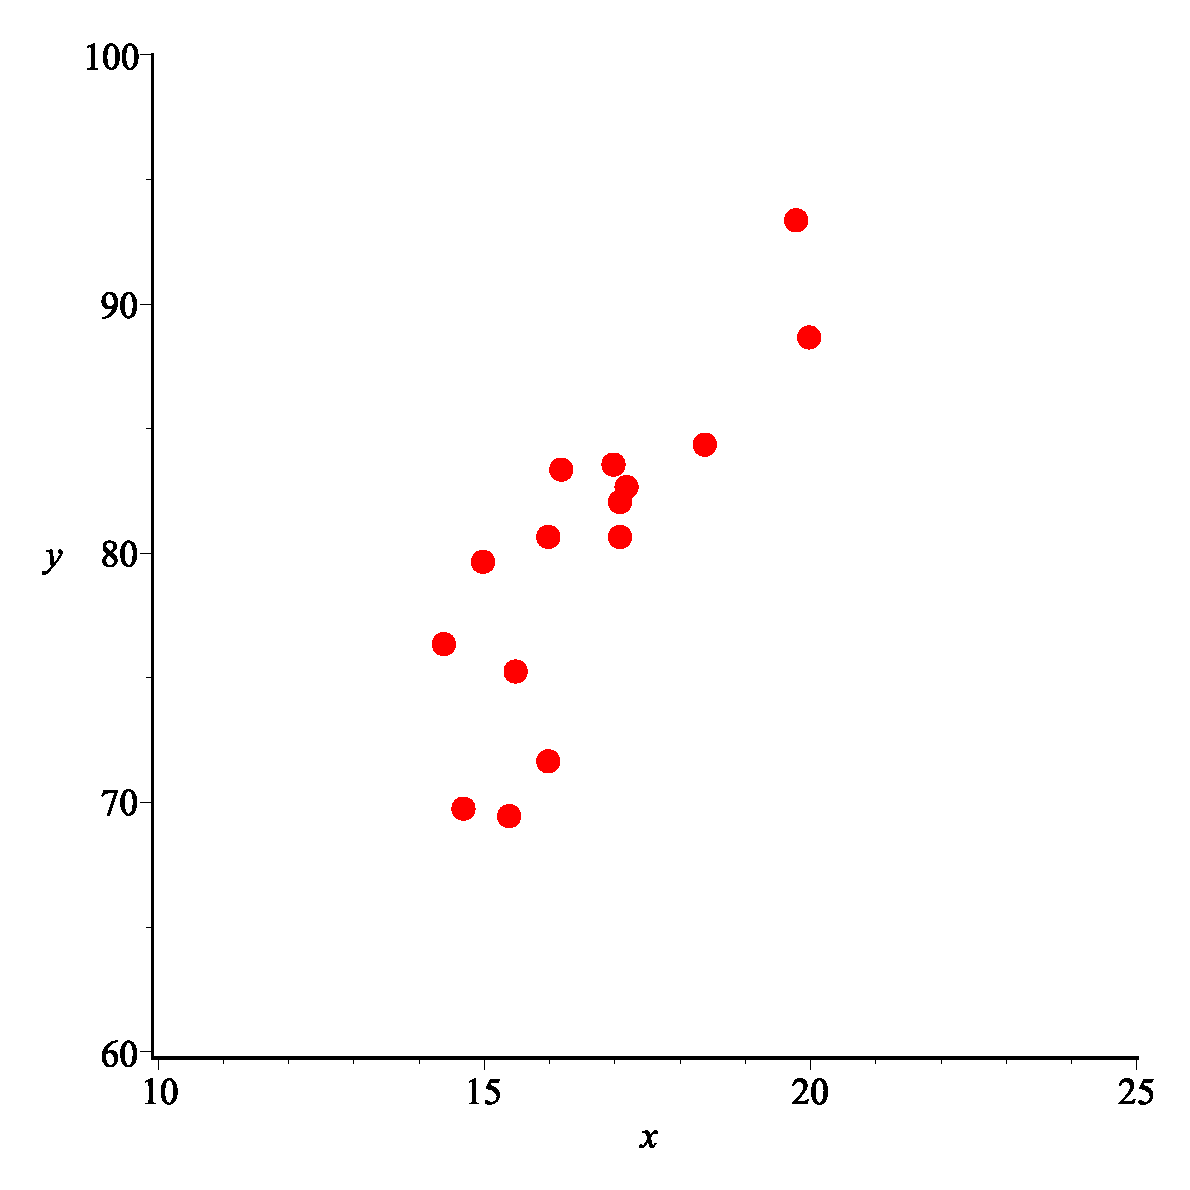
\includegraphics{figures/fig_10_7_crickets.eps}}
    \end{center}

If we want to use the data to make predications, then we need to fit a curve of some kind to the data. Since the cricket data appears roughly linear, we will fit a linear function $f$ of the form $f(x) = mx+b$ to the data. We will do this in such a way that we minimize the sums of the squares of the distances between the $y$ values of the data and the corresponding $y$ values of the line defined by $f$. This type of fit is called a \emph{least squares} approximation. If the data is represented by the points $(x_1,y_1)$, $(x_2,y_2)$, $\ldots$, $(x_n,y_n)$, then the square of the distance between $y_i$ and $f(x_i)$ is $(f(x_i)-y_i)^2 = (mx_i+b-y_i)^2$. So our goal is to minimize the sum of these squares, of minimize the function $S$ defined by 
\[S(m,b) = \sum_{i=1}^n (mx_i+b-y_i)^2.\]
\ba
\item Calculate $S_m$ and $S_b$.

\item Solve the system $S_m(m,b) = 0$ and $S_b(m,b) = 0$ to show that the critical point satisfies 
\begin{align*}
m &= \frac{n\left(\sum_{i=1}^n x_iy_i\right) - \left(\sum_{i=1}^n x_i \right) \left(\sum_{i=1}^n y_i \right)}{n\left(\sum_{i=1}^n x_i^2 \right) - \left(\sum_{i=1}^n x_i \right)^2} \\
b &= \frac{\left(\sum_{i=1}^n y_i\right) \left(\sum_{i=1}^n x_i^2\right) - \left(\sum_{i=1}^n x_i \right) \left(\sum_{i=1}^n x_iy_i \right)}{n\left(\sum_{i=1}^n x_i^2 \right) - \left(\sum_{i=1}^n x_i \right)^2}.
\end{align*}
(Hint: Don't be daunted by these expressions, the system $S_m(m,b) = 0$ and $S_b(m,b) = 0$ is a system of two linear equations in the unknowns $m$ and $b$. It might be easier to let $r=\sum_{i=1}^n x_i^2$, $s=\sum_{i=1}^n x_i$, $t = \sum_{i=1}^n y_i$, and $u = \sum_{i=1}^n x_iy_i$ and write your equations using these constants.)

\item Use the Second Derivative Test to explain why the critical point gives a local minimum. Can you then explain why the critical point gives an absolute minimum? 

\item Use the formula from part (b) to find the values of $m$ and $b$ that give the line of best fit in the least squares sense to the cricket data. Draw your line on the scatter plot to convince yourself that you have a well-fitting line. 

\ea

\begin{exerciseSolution}
\ba
\item We are assuming that the only variables are $m$ and $b$. With 
\[S(m,b) = \sum_{i=1}^n (mx_i+b-y_i)^2 = (mx_1+b-y_1)^2 + (mx_2+b-y_2)^2 + \cdots + (mx_n+b-y_n)^2\]
we have 
\[S_m(m,b) =  \sum_{i=1}^n 2x_i(mx_i+b-y_i) \ \text{ and } \ S_b(m,b) = \sum_{i=1}^n 2(mx_i+b-y_i).\]

\item We want to solve the system  
\begin{align*}
0 &= \sum_{i=1}^n 2x_i(mx_i+b-y_i) = 2x_1(mx_1+b-y_1) + 2x_2(mx_2+b-y_2) + \cdots + 2x_n(mx_n+b-y_n) \\	
	&= \left(m\sum_{i=1}^n 2x_i^2\right) + \left(b \sum_{i=1}^n 2x_i \right) - \left(\sum_{i=1}^n 2x_iy_i \right) \\
0 &= \sum_{i=1}^n 2(mx_i+b-y_i) = 2(mx_1+b-y_1) + 2(mx_2+b-y_2) + \cdots + 2(mx_n+b-y_n) \\
	&= \left(m\sum_{i=1}^n 2x_i\right) + 2nb - \left(\sum_{i=1}^n 2y_i\right)
\end{align*}
for $m$ and $b$. To simplify the work, let $r=\sum_{i=1}^n x_i^2$, $s=\sum_{i=1}^n x_i$, $t = \sum_{i=1}^n y_i$, and $u = \sum_{i=1}^n x_iy_i$. Our system then has the form
\begin{align}
0 &= 2mr + 2bs -2u \label{eq:10_7_crickets_1} \\
0 &= 2ms + 2nb - 2t. \label{eq:10_7_crickets_2}
\end{align}
Multiplying both sides of equation (\ref{eq:10_7_crickets_2}) by r and equation (\ref{eq:10_7_crickets_1}) by $s$ and subtracting corresponding sides gives us 
\[0 = 2bs^2-2us-2nbr+2tr = 2b(s^2-nr) - 2(us-tr).\]
Solving for $b$ yields
\[b = \frac{tr-us}{nr-s^2} = \frac{\left(\sum_{i=1}^n y_i\right) \left(\sum_{i=1}^n x_i^2\right) - \left(\sum_{i=1}^n x_i \right) \left(\sum_{i=1}^n x_iy_i \right)}{n\left(\sum_{i=1}^n x_i^2 \right) - \left(\sum_{i=1}^n x_i \right)^2}.\]
If instead we multiply both sides equation (\ref{eq:10_7_crickets_2}) by $s$ and both sides of equation (\ref{eq:10_7_crickets_1}) by $n$ and subtract corresponding sides we get 
\[0 = 2nmr-2ms^2-2nu+2ts = 2m(nr-s^2)-2(nu-ts).\]
 Solving for $m$ gives us 
\[m=\frac{nu-ts}{nr-s^2} = \frac{n\left(\sum_{i=1}^n x_iy_i\right) - \left(\sum_{i=1}^n x_i \right) \left(\sum_{i=1}^n y_i \right)}{n\left(\sum_{i=1}^n x_i^2 \right) - \left(\sum_{i=1}^n x_i \right)^2}.\]


\item The second order partial derivatives of $S$ are 
\[S_m(m,b) =  \sum_{i=1}^n 2x_i(mx_i+b-y_i) \ \text{ and } \ S_b(m,b) = \sum_{i=1}^n 2(mx_i+b-y_i).\]
\[S_{mm}(m,b) = \sum_{i=1}^n 2x_i^2, \ S_{bb}(m,b) = \sum_{i=1}^n 2 = 2n, \ \text{ and } \ S_{mb}(m,b) = \sum_{i=1}^n 2x_i.\]
For our data, $n=15$, $\sum_{i=1}^n x_i^2 = 4200.56$, and $\sum_{i=1}^n x_i = 249.8$, so 
\[S_{mm}(x,y)S_{bb}(x,y) - S_{mb}(x,y)^2 = 2n\left(\sum_{i=1}^n 2x_i^2\right)- \left(\sum_{i=1}^n 2x_i\right)^2 = 2433.44.\]
Since $S_{mm}(m,b) = \sum_{i=1}^n 2x_i^2 > 0$, it follows that this critical point is a local minimum. Note that the discriminant is a constant, as is $S_{mm}(m,b)$, so the surface defined by $S$ is always concave up, giving us an absolute minimum at this critical point. 
 
\item Using the formula from part (b), we find that $m \approx 3.291094089$ and $b \approx 25.2323131$, giving us the best fit line $y = 3.291094089x + 25.2323131$. a plot of this line against the data shows a pretty good linear fit. 

\ea
\end{exerciseSolution}


\end{exercises}
\afterexercises
